\chapter{Esempi d'uso e risultato}
\label{sec:Esempi d'uso e risultato}

\section[Parametri utilizzati]{Parametri utilizzati} % ok with fontsize=12pt
Sono state effettuate cinque diverse simulazione. Le prime tre simulazioni sono state effettuate senza effettuare variazioni. La quarta simulazione è stata effettuata dopo aver scambiato la scuderia di due piloti; il pilota "Lewis Hamilton" della scuderia "Mercedes" è stato scambiato con il pilota "Carlos Sainz" della scuderia "McLaren". La quinta e ultima simulazione è invece stata effettuata dopo aver investito nella scuderia "Ferrari" un quantitativo di milioni di euro pari a trecento.
\begin{figure}[h]
\centering
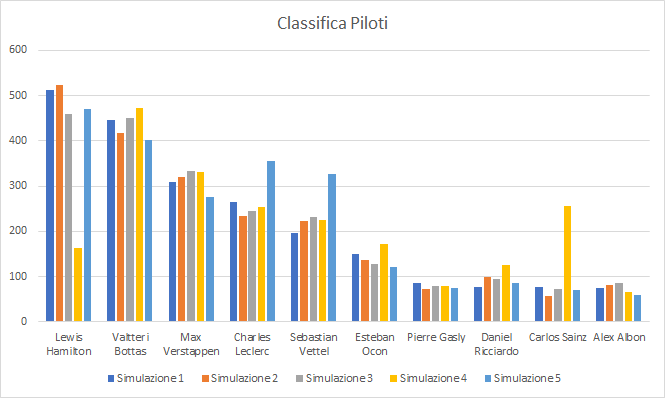
\includegraphics[width=0.9\linewidth]{images/classifica Piloti1.png}
\caption{Classifica Piloti in diverse simulazioni}
\label{fig:Classifica Piloti in diverse simulazioni}
\end{figure}
\begin{figure}[h]
\centering
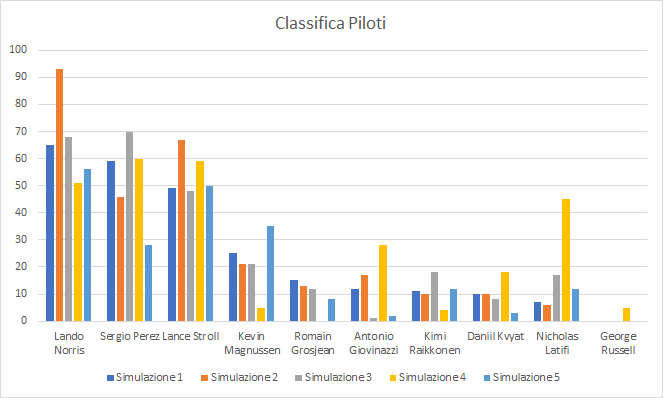
\includegraphics[width=0.9\linewidth]{images/classifica Piloti2.png}
\caption{Classifica Piloti in diverse simulazioni}
\label{fig:Classifica Piloti in diverse simulazioni}
\end{figure}
\begin{figure}[h]
\centering
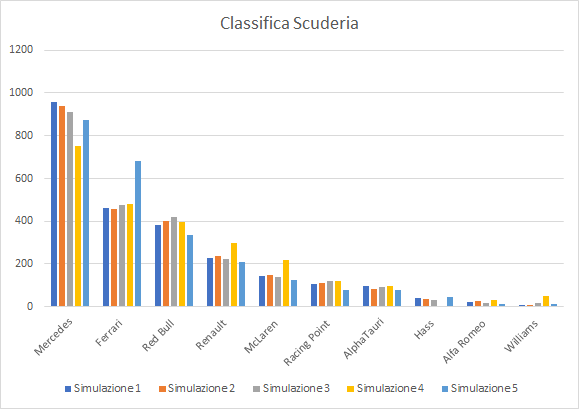
\includegraphics[width=0.9\linewidth]{images/Classifica Scuderia.png}
\caption{Classifica Scuderia in diverse simulazioni}
\label{fig:Classifica Scuderia in diverse simulazioni}
\end{figure}
\clearpage
\section[Analisi]{Analisi} % ok with fontsize=12pt

Dalle figure 7.1, 7.2 e 7.3 è possibile analizzare i risultati delle diverse simulazioni. Come era facilmente pronosticabile il campione del mondo risulta per quattro volte su cinque "Lewis Hamilton" poichè egli ha il punteggio abilità più elevato tra i piloti in griglia, guida la macchina con il punteggio più alto e negli anni precedenti ha ottenuto i migliori tempi. É importante notare che nella figura 7.2 i punteggi dei piloti siano scalati graficamente sul punteggio del pilota che occupa l'undicesima posizione nella prima simulazione. Nella quarta simulazione possiamo osservare gli evidenti effetti di uno scambio di vettura tra due piloti di due scuderie diverse; in questo caso possiamo notare come i due piloti tendano a variare le loro posizioni finali in base alla differenza di punteggio assegnato alle due vetture. Nell'ultima simulazione invece si può vedere come i due piloti della scuderia "Ferrari": "Charles Leclerc" e "Sebastian Vettel" riescano a colmare il gap con "Max Verstappen" ma non il gap con i primi due piloti, entrambi della scuderia "Mercedes"; questo avviene poichè prima della simulazione numero cinque sono stati aumentati i fondi alla scuderia "Ferrari" di un ammontare di milioni pari a trecento e quindi del conseguente miglioramento dei tempi di percorrenza dei giri e del punteggio assegnato alla vettura.\\
Per concludere, una breve riflessione sui dati generati dalle simulazioni. Seppur le simulazioni includono delle variabili aleatorie, i dati che esse producono sono affetti da una notevole dipendenza dei dati delle stagioni passate. Questo si ripercuote sulla poca variabilità delle posizioni finali dei primi classificati; è facilmente intuibile dalle figure 7.2 e 7.3 come la parte centrale della classifica è più affetta a variabilità sia in termini di punteggi finali sia in termini di posizioni questo poichè i punteggi delle vetture, dei piloti e i tempi di giri sono molto vicini tra loro e dunque le variabili casuali tendono a disordinare le posizioni finali dei piloti.
\clearpage

\begin{figure}[h]
\centering
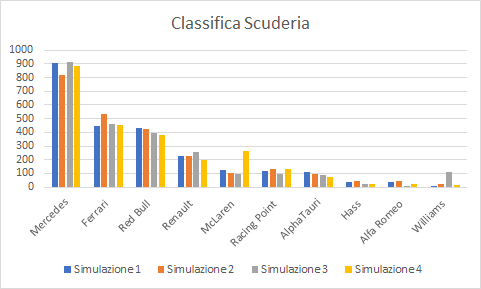
\includegraphics[width=0.9\linewidth]{images/Classifica Scuderia nuovo pilota.png}
\caption{Classifica Scuderia dopo l'introduzione di un nuovo pilota}
\label{fig:Classifica Scuderia dopo l'introduzione di un nuovo pilota}
\end{figure}
\begin{figure}[h]
\centering
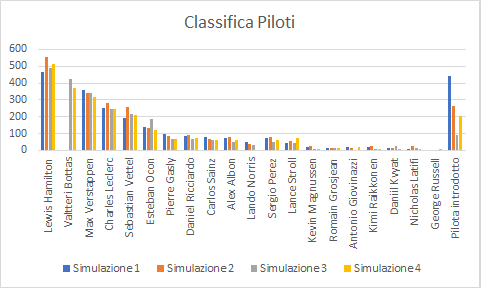
\includegraphics[width=0.9\linewidth]{images/Classifica Piloti Nuovo Pilota.png}
\caption{Classifica Piloti dopo l'introduzione di un nuovo pilota}
\label{fig:CClassifica Piloti dopo l'introduzione di un nuovo pilota}
\end{figure}
\clearpage
\section[Parametri introduzione nuovo pilota]{Parametri introduzione nuovo pilota} % ok with fontsize=12pt
Sono state effettuate quattro diverse simulazione. Al pilota introdotto è stato modificato il punteggio abilità nel corso delle diverse simulazioni ed è variato il pilota sostituito così da poter cercare di analizzare l'influenza che il punteggio abilità e la scuderia scelta hanno sulla simulazione del campionato.
\begin{enumerate}
    \item il pilota introdotto ha il punteggio abilità massimo (99) e viene scambiato con il secondo pilota con il punteggio più alto e introdotto nella scuderia "Mercedes" che risulta la scuderia con il punteggio più alto;
    \item il pilota introdotto ha un punteggio abilità simile a quello del pilota con il punteggio più basso in griglia (70) e viene scambiato con il secondo pilota con il punteggio più alto e introdotto nella scuderia "Mercedes" che risulta la scuderia con il punteggio più alto;
    \item il pilota introdotto ha un punteggio abilità nella media dei punteggi dei piloti in griglia (85) e viene scambiato con il pilota con il punteggio più basso e introdotto nella scuderia "Williams" che risulta la scuderia con il punteggio più basso;
    \item il pilota introdotto ha un punteggio abilità nella media dei punteggi dei piloti in griglia (85) e viene scambiato con un pilota che ha un punteggio minore e introdotto nella scuderia "McLaren" che risulta una scuderia che ha un punteggio nella media.
    \end{enumerate}
\section[Analisi]{Analisi} % ok with fontsize=12pt

Dalle figure 7.4 e 7.5 è possibile analizzare i risultati delle diverse simulazioni. Nella prima simulazione è importante notare come il campionato venga vinto da "Lewis Hamilton" anche se il pilota introdotto guida la stessa vettura ed ha un punteggio abilità più alto; questo è dovuto al fatto che la diffferenza dei tempi tra "Lewis Hamilton" e il pilota eliminato "Valtteri Bottas" non è spiegata solamente dalla differenza di abilità dei due piloti. Il pilota introdotto risulta comunque secondo al termine del campionato. Nella seconda simulazione il pilota viene introdotto con un punteggio abilità molto basso e questo fa sì che il pilota introdotta raggiunga soltanto la quarta posizione seppur avendo la migliore vettura. Nella simulazione 3 viene introdotto un pilota con un punteggio medio nella scuderia che prima dello scambio risultava ultima nelle diverse simulazioni effettuate in precedenza e in 7.1 e 7.2. In questo caso il pilota raggiunge la settima posizione e questo poichè la differenza tra il pilota eliminato e quello introdotto è molto elevata. Nell'ultima simulazione il pilota è introdotto con punteggio medio e al posto di un pilota con punteggio minore. Addizionando a questa differenza di abilità, il posizionamento della scuderia nella parte centrale della classifica, ovvero quella soggetta a più variazione in presenza di nuovi fattori, il pilota introdotto raggiunge la sesta posizione e quindi vi è un netto miglioramento nel posizionamento della scuderia "McLaren" nel campionato costruttori.